\documentclass{article}

\usepackage{graphicx}
\usepackage{tikz}
\usepackage{tikzsymbols}
\usetikzlibrary{calc,patterns,shapes.geometric}
\pagestyle{empty}
\usepackage[margin=0pt]{geometry}
\geometry{papersize={14in,12in}}

\def\centerarc[#1](#2)(#3:#4:#5){\draw[#1] ($(#2)+({#5*cos(#3)},{#5*sin(#3)})$) arc (#3:#4:#5);}

\begin{document}
	\begin{figure}
		\centering
		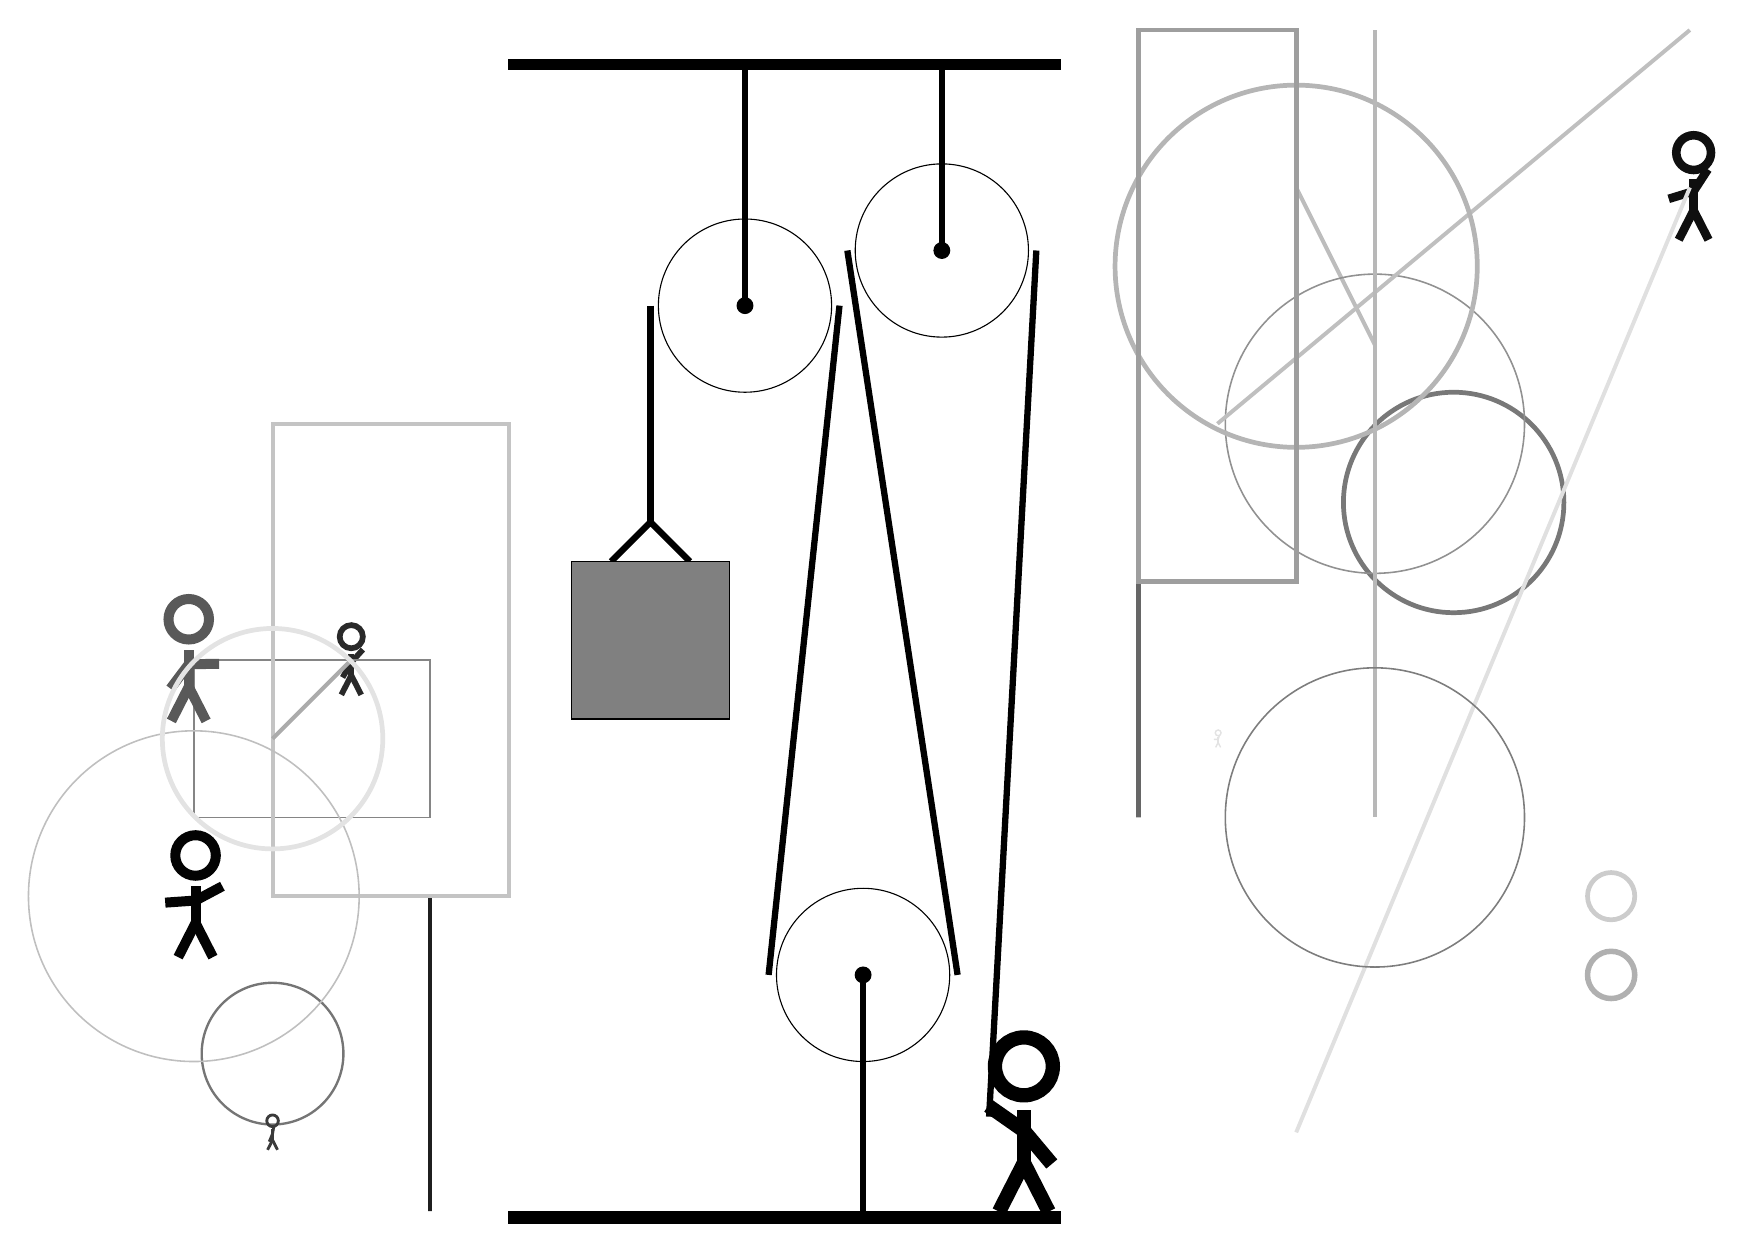
\begin{tikzpicture}
			%%%%% START %%%%%
			
			\draw[fill=black] (-2, 11.5) rectangle (5, 11.625);
			
			\draw[line width=0.4mm, color=black!88] (-3, -3) rectangle (-3, 1);
			
			\node[line width=0.3mm, color=black!84] at (-4, 4) {\Strichmaxerl[4][60][48]};
			\draw[line width=0.2mm, color=black!48] (-3, 2) rectangle (-6, 4);
			\draw[line width=0.5mm, color=black!23] (-2, 7) rectangle (-5, 1);
			\node[line width=0.3mm, color=black!11] at (7, 3) {\Strichmaxerl[1][1][72]};
			
			\node[line width=0.3mm, color=black!94] at (13, 10) {\Strichmaxerl[6][17][57]};
			
			\draw [line width=0.7mm, color=black!31](12, 0) circle (0.3);
			\node[line width=0.6mm, color=black!99] at (-6, 1) {\Strichmaxerl[7][4][28]};
			\draw[line width=0.5mm, color=black!26](9, 8) -- (8, 10);
			\draw [line width=0.6mm, color=black!53](10, 6) circle (1.4);
			\draw [line width=0.3mm, color=black!54](-5, -1) circle (0.9);
			\draw[line width=0.5mm, color=black!12](8, -2) -- (13, 10);
			\draw[line width=0.7mm, color=black!60] (6, 11) rectangle (6, 2);
			
			\draw [line width=0.2mm, color=black!43](9, 7) circle (1.9);
			\draw[line width=0.5mm, color=black!25](7, 7) -- (13, 12);
			\draw [line width=0.6mm, color=black!29](8, 9) circle (2.3);
			\draw[line width=0.6mm, color=black!38] (6, 5) rectangle (8, 12);
			\draw [line width=0.6mm, color=black!20](12, 1) circle (0.3);
			\draw[line width=0.5mm, color=black!28](9, 12) -- (9, 2);
			\node[line width=0.7mm, color=black!65] at (-6, 4) {\Strichmaxerl[7][53][1]};
			\draw[line width=0.5mm, color=black!33](-4, 4) -- (-5, 3);
			\node[line width=0.2mm, color=black!77] at (-5, -2) {\Strichmaxerl[2][68][80]};
			\draw [line width=0.2mm, color=black!25](-6, 1) circle (2.1);
			\draw [line width=0.6mm, color=black!11](-5, 3) circle (1.4);
			\draw [line width=0.2mm, color=black!51](9, 2) circle (1.9);
			
			\draw (1, 8.5) circle (1.1);
			\draw[fill=black] (1, 8.5) circle (0.1);
			\draw[line width=0.8mm]  (1, 11.5) -- (1, 8.5);
			
			\draw[fill=white](2.5, 0.0) circle (1.1);
			\draw[fill=black] (2.5, 0.0) circle (0.1);
			\draw[line width=0.8mm]  (2.5, -3) -- (2.5, 0.0);
			
			\draw[fill=white](3.5, 9.2) circle (1.1);
			\draw[fill=black] (3.5, 9.2) circle (0.1);
			\draw[line width=0.8mm] (3.5, 11.5) -- (3.5, 9.2);
			
			\draw[line width=0.8mm] (-0.7, 5.25) -- (-0.2, 5.75) -- (0.3, 5.25);
			\draw[fill=black!50] (-1.2, 5.25) rectangle (0.8, 3.25);
			
			\draw[line width=0.8mm] (-0.2, 8.5) -- (-0.2, 5.75);
			\centerarc[line width=0.8mm](1, 8.5)(0:180:1.2000000000000002);
			\draw[line width=0.8mm](2.2, 8.5) -- (1.3, 0.0);
			\centerarc[line width=0.8mm](2.5, 0.0)(180:360:1.2000000000000002);
			\draw[line width=0.8mm](3.7, 0.0) -- (2.3, 9.2);
			\centerarc[line width=0.8mm](3.5, 9.2)(0:180:1.2000000000000002);
			\draw[line width=0.8mm](4.7, 9.2) -- (4.1, -1.8);
			
			\node at (4.5, -1.9) {\Strichmaxerl[10][-35][-50]};
			
			\draw[fill=black] (-2, -3) rectangle (5, -3.15);
			
			%%%%% END %%%%%
		\end{tikzpicture}
	\end{figure}	
\end{document}